\documentclass[sigconf]{acmart}

\usepackage{booktabs} % For formal tables

\usepackage{amsmath}
\usepackage{float}
\usepackage{hyperref}
\usepackage{listings}
\usepackage{algorithm}
\usepackage[noend]{algpseudocode}
\usepackage{graphicx}
\usepackage{courier}
\usepackage{float}
\usepackage{color}
\usepackage[margin=10pt,font=small,labelfont=bf,
  labelsep=endash]{caption}
\usepackage{ulem}

\usepackage{syntax} % for writing BNF grammar

\usepackage{forest}
\usepackage{framed}

\usepackage{tikz}
\usetikzlibrary{matrix}
\usetikzlibrary{shapes.multipart}
\usetikzlibrary{patterns}
\usetikzlibrary{positioning,fit,calc}
\usetikzlibrary{decorations.pathmorphing}
\usetikzlibrary{decorations.pathreplacing}
\usetikzlibrary{quotes}
\usetikzlibrary{graphs}
\usetikzlibrary{arrows.meta}
\usetikzlibrary{shapes}
% \usetikzlibrary{graphs,graphdrawing}
% \usegdlibrary{layered}
% \usetikzlibrary{graphdrawing,graphs,calc}
% \usegdlibrary{layered}

\usepackage{smartdiagram}

% \usetikzlibrary{external}
% \tikzexternalize % activate!
% \tikzset{external/force remake}

%% To generate figure, uncomment above three lines, and execute:
%% pdflatex -shell-escape helium.tex

\usepackage{csvsimple}
\usepackage{multirow}


\lstset{basicstyle=\footnotesize\ttfamily,breaklines=true}
% \lstset{frame=b}
\lstset{float,floatplacement=H,captionpos=b}
% \lstset{numbers=left}
\lstset{language=C}
\lstset{showstringspaces=false}
\lstset{breakindent=10pt}
% \lstset{framextopmargin=10pt}
% \lstset{framextopmargin=50pt,frame=t}
% \lstset{float=htb,language=C,frame=single, basicstyle=\small, stringstyle=\ttfamily}
% \lstset{escapeinside={(*@}{@*)}}
% \usepackage{xcolor}
\lstdefinestyle{base}{
  language=C,
  emptylines=1,
  breaklines=true,
  aboveskip=0em,
  belowskip=0em,
  % float,
  % floatplacement=H,
  basicstyle=\footnotesize\ttfamily\color{black},
  moredelim=**[is][\color{blue}]{@}{@},
  moredelim=**[is][\color{purple}]{~1}{~1},
  moredelim=**[is][\color{brown}]{~2}{~2},
  moredelim=**[is][\color{gray}]{~3}{~3},
  moredelim=**[is][\color{orange}]{~4}{~4},
  moredelim=**[is][\color{violet}]{~5}{~5},
}
\lstdefinestyle{graycode} {
  language=C,
  emptylines=1,
  breaklines=true,
  basicstyle=\footnotesize\ttfamily\color{gray!50},
  moredelim=**[is][\color{blue}]{@}{@},
}
\lstset{style=base}




\begin{document}

\title{Test}



\begin{figure*}
  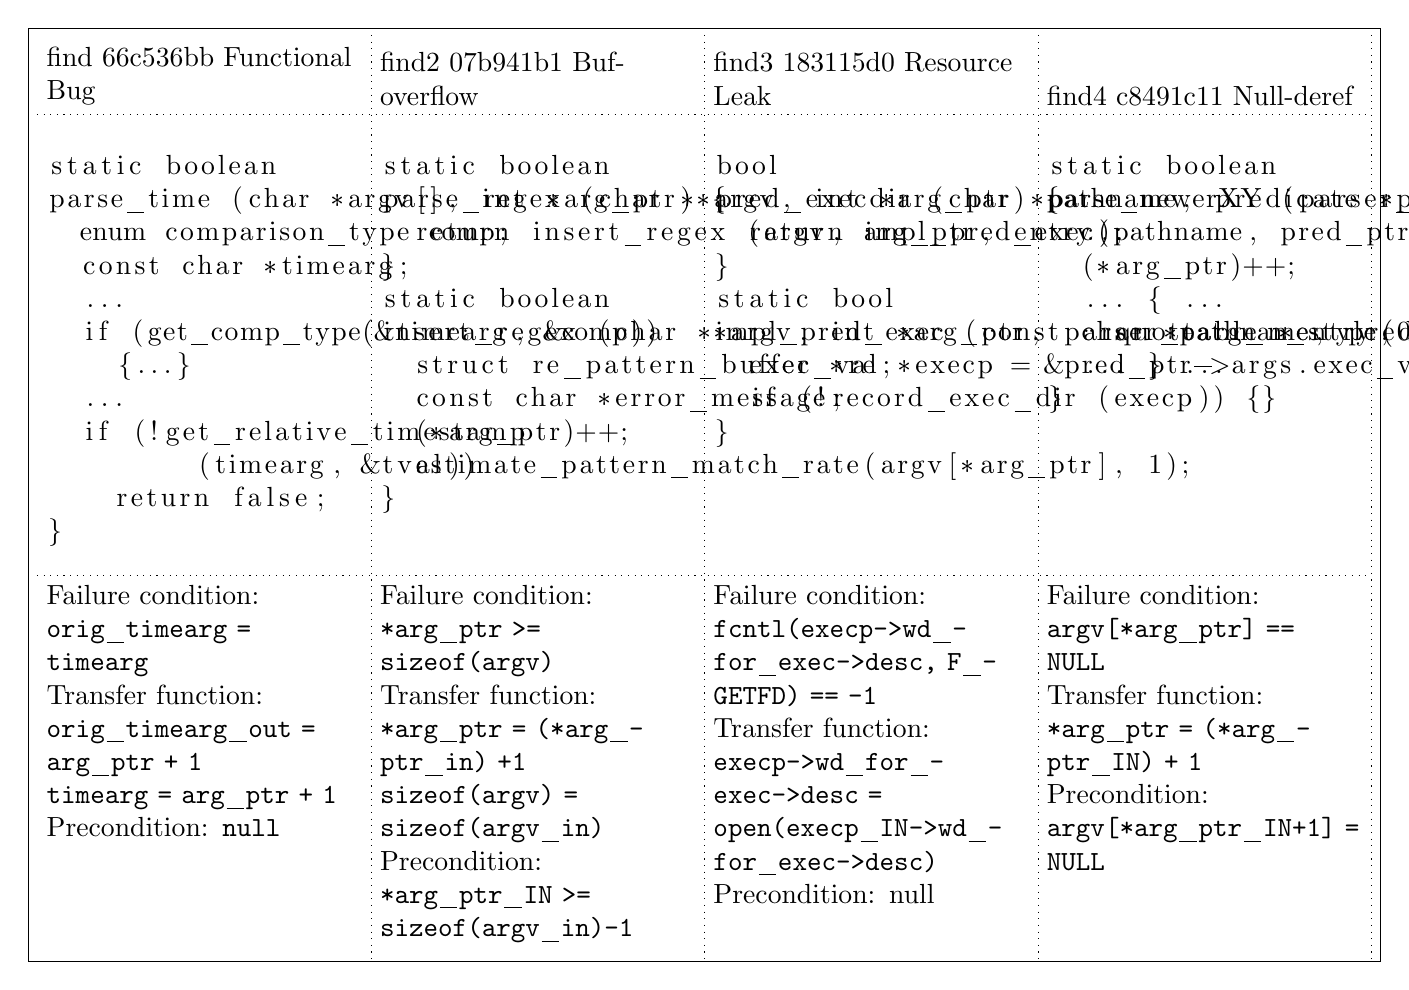
\begin{tikzpicture}
    \matrix (m) [
      draw,
      matrix anchor=north,
      every node/.style={
        % draw,
        anchor=north west, text width=4cm}] {
      \node (c1) ["find 66c536bb Functional Bug"]{
        \begin{lstlisting}
static boolean 
parse_time (char *argv[], int *arg_ptr) {
  enum comparison_type comp;
  const char *timearg;
  ...
  if (get_comp_type(&timearg, &comp))
    {...}
  ...
  if (!get_relative_timestamp
         (timearg, &tval))
    return false;
}
\end{lstlisting}
      };&
      \node (c2) ["find2 07b941b1 Buf-overflow"] {
        \begin{lstlisting}
static boolean
parse_regex (char **argv, int *arg_ptr) {
  return insert_regex (argv, arg_ptr, entry);
}
static boolean
insert_regex (char **argv, int *arg_ptr, parser_table *entry, int regex_options) {
  struct re_pattern_buffer *re;
  const char *error_message;
  (*arg_ptr)++;
  estimate_pattern_match_rate(argv[*arg_ptr], 1);
}
\end{lstlisting}
      };&
      \node (c3) ["find3 183115d0 Resource Leak"] {
        \begin{lstlisting}
bool
pred_execdir (char *pathname, predicate *pred_ptr) {
  return impl_pred_exec(pathname, pred_ptr);
}
static bool
impl_pred_exec (const char *pathname, predicate *pred_ptr) {
  exec_val *execp = &pred_ptr->args.exec_vec;
  if (!record_exec_dir (execp)) {}
}
\end{lstlisting}
      };&
      \node (c4) ["find4 c8491c11 Null-deref"] {
        \begin{lstlisting}
static boolean
parse_newerXY (parser_table* entry, char **argv, int *arg_ptr) {
  ...
  (*arg_ptr)++;
  ... { ...
    quotearg_n_style(0, options.err_quoting_style, argv[*arg_ptr]);
  ... } ...
}
\end{lstlisting}
      };\\
      \node (f1) {
        Failure condition:\\
        \texttt{orig_timearg = timearg}\\
        Transfer function:\\
        \texttt{orig_timearg_out = arg_ptr + 1}\\
        \texttt{timearg = arg_ptr + 1}\\
        Precondition: \texttt{null}\\
      };&
      \node (f2) {
        Failure condition:\\
        \texttt{*arg_ptr >= sizeof(argv)}\\
        Transfer function:\\
        \texttt{*arg_ptr = (*arg_ptr_in) +1}\\
        \texttt{sizeof(argv) = sizeof(argv_in)}\\
        Precondition: \texttt{*arg_ptr_IN >= sizeof(argv_in)-1}
      };&
      \node (f3) {
        Failure condition:\\
        \texttt{fcntl(execp->wd_for_exec->desc, F_GETFD) == -1}\\
        Transfer function:\\
        \texttt{execp->wd_for_exec->desc = open(execp_IN->wd_for_exec->desc)}\\
        Precondition: null\\
      };&
      \node (f4) {
        Failure condition:
        \texttt{argv[*arg_ptr] == NULL}\\
        Transfer function:
        \texttt{*arg_ptr = (*arg_ptr_IN) + 1}\\
        Precondition:
        \texttt{argv[*arg_ptr_IN+1] = NULL}\\
      };\\
    };
    \draw [dotted] (c1.north west) -- (c4.north east);
    \draw [dotted] (f1.north west) -- (f4.north east);
    \foreach \x in {1,2,3,4}
    \draw [dotted] (c\x.north east |- m.north) -- (f\x.south east |- m.south);
  \end{tikzpicture}
  \caption{Bug signature of four types}
\end{figure*}

\end{document}
